% Chapter Template

\chapter{Analysis} % Main chapter title

\label{Analysis} % Change X to a consecutive number; for referencing this chapter elsewhere, use \ref{ChapterX}

%----------------------------------------------------------------------------------------
%	SECTION 1
%----------------------------------------------------------------------------------------

The analysis results in a domain model, containing entities discovered from the requirements. These entities are obtained through a noun-analysis on the functional requirements and provides an overview of abstract concepts within the system.\\
The communication flow between the system and its users was analyzed. This resulted in an abstract version of the API.

\section{Domain model}
\begin{figure}[H]
	\centering
	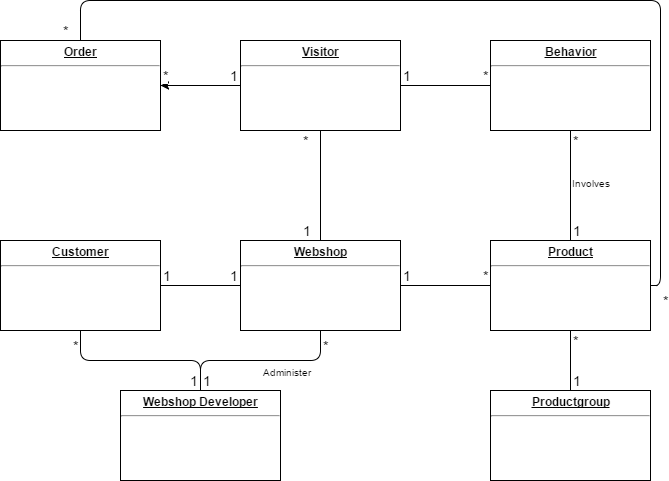
\includegraphics[width=.8\linewidth]{Figures/Domain_model.png}
	\caption{Domain model}
	\label{fig:DomainModel}
\end{figure}

The domain model in figure \ref{fig:DomainModel} is the result of the analysis of the requirements. The domain model provides an overview of concepts in the system, and how they are related.

\begin{description}
	\item[Webshop Developer] is the company developing and hosting a collection of webshops. In this project the Webshop Developer is the company Struct A/S, who wish to add value to their services by offering product recommendations. Seen from the perspective of the project group, this is the customer who ordered a recommendation system.
	\item[Customer] is an owner of a webshop, developed by the Webshop Developer. Customer is a secondary stakeholder that desires the possibility of presenting product recommendations to its visitors.
	\item[Webshop] is the webshop owned by a customer, and developed and hosted by the Webshop Developer. Webshop offers a variety of products and presents them to the visitors of the site.
	\item[Visitor] is the end-user of the webshop. This is a potential customer to the owner of the webshop and will have product recommendations presented once the recommendation system is applied.
	\item[Product] is the different products available for purchase on the webshop. 
	\item[Productgroup] is the distinction between groups of products.
	\item[Behavior] describes an action of Visitor on the webshop. If a visitor clicks on a product, this is considered a Behavior. 
\end{description}

\section{API}
The API of the system is essential for making the product recommendation system available to the Webshop Developer. The following calls to the API were identified from analyzing the requirements:

\begin{description}
	\item[GetProductRecommendations] allows the client to ask for product recommendations to a Visitor.
	\item[StoreBehavior] stores new behavior in the system.
	\item[DeleteBehavior] deletes existing behavior from the system.
	\item[StoreVisitor] stores a new Visitor in the system.
	\item[UpdateVisitor] updates information about an existing Visitor in the system.
	\item[DeleteVisitor] deletes an existing Visitor from the system.
	\item[StoreProduct] stores a new Product in the system.
	\item[UpdateProduct] updates information about an existing Product in the system.
	\item[DeleteProduct] deletes an existing Product from the system.
	\item[StoreOrder] stores a new order in the system.
	\item[DeleteOrder] deletes an existing order from the system.
\end{description}

The discovered API calls indicates that the system will consist of two aspects, data management and product recommendations.\\
Combining the domain model and the API calls grants an overview of the concepts and their relations within the system. 